
\begin{figure} [H]
\begin{center} 
\tikzset{every picture/.style={line width=0.75pt}} %set default line width to 0.75pt        

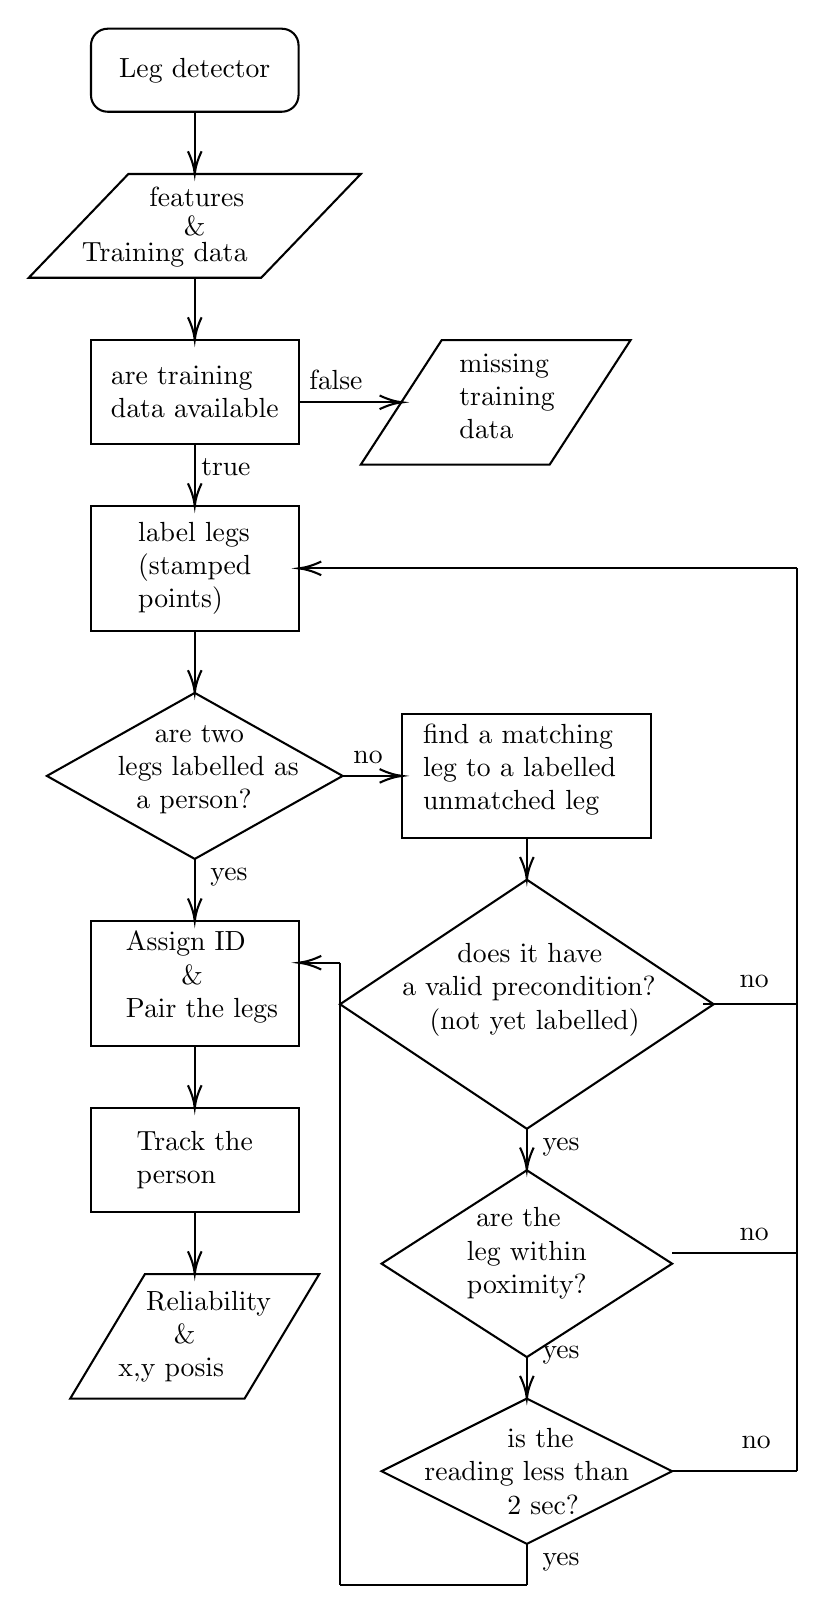
\begin{tikzpicture}[x=0.75pt,y=0.75pt,yscale=-1,xscale=1]
%uncomment if require: \path (0,811); %set diagram left start at 0, and has height of 811

%Rounded Rect [id:dp2960782928568111] 
\draw   (270,38) .. controls (270,33.58) and (273.58,30) .. (278,30) -- (362,30) .. controls (366.42,30) and (370,33.58) .. (370,38) -- (370,62) .. controls (370,66.42) and (366.42,70) .. (362,70) -- (278,70) .. controls (273.58,70) and (270,66.42) .. (270,62) -- cycle ;
%Straight Lines [id:da8889190192256218] 
\draw    (320,70) -- (320,98) ;
\draw [shift={(320,100)}, rotate = 270] [color={rgb, 255:red, 0; green, 0; blue, 0 }  ][line width=0.75]    (10.93,-3.29) .. controls (6.95,-1.4) and (3.31,-0.3) .. (0,0) .. controls (3.31,0.3) and (6.95,1.4) .. (10.93,3.29)   ;

%Shape: Parallelogram [id:dp4552473223976452] 
\draw   (288,100) -- (400,100) -- (352,150) -- (240,150) -- cycle ;
%Shape: Rectangle [id:dp7650580320202618] 
\draw   (270,180) -- (370,180) -- (370,230) -- (270,230) -- cycle ;
%Straight Lines [id:da15946321526077067] 
\draw    (320,150) -- (320,178) ;
\draw [shift={(320,180)}, rotate = 270] [color={rgb, 255:red, 0; green, 0; blue, 0 }  ][line width=0.75]    (10.93,-3.29) .. controls (6.95,-1.4) and (3.31,-0.3) .. (0,0) .. controls (3.31,0.3) and (6.95,1.4) .. (10.93,3.29)   ;

%Straight Lines [id:da5115795703209409] 
\draw    (320,230) -- (320,258) ;
\draw [shift={(320,260)}, rotate = 270] [color={rgb, 255:red, 0; green, 0; blue, 0 }  ][line width=0.75]    (10.93,-3.29) .. controls (6.95,-1.4) and (3.31,-0.3) .. (0,0) .. controls (3.31,0.3) and (6.95,1.4) .. (10.93,3.29)   ;

%Straight Lines [id:da42832604352700177] 
\draw    (370,210) -- (418,210) ;
\draw [shift={(420,210)}, rotate = 180] [color={rgb, 255:red, 0; green, 0; blue, 0 }  ][line width=0.75]    (10.93,-3.29) .. controls (6.95,-1.4) and (3.31,-0.3) .. (0,0) .. controls (3.31,0.3) and (6.95,1.4) .. (10.93,3.29)   ;

%Shape: Parallelogram [id:dp7391100262642236] 
\draw   (439,180) -- (530,180) -- (491,240) -- (400,240) -- cycle ;
%Shape: Rectangle [id:dp3821183545244151] 
\draw   (270,260) -- (370,260) -- (370,320) -- (270,320) -- cycle ;
%Straight Lines [id:da19529012230832055] 
\draw    (320,320) -- (320,348) ;
\draw [shift={(320,350)}, rotate = 270] [color={rgb, 255:red, 0; green, 0; blue, 0 }  ][line width=0.75]    (10.93,-3.29) .. controls (6.95,-1.4) and (3.31,-0.3) .. (0,0) .. controls (3.31,0.3) and (6.95,1.4) .. (10.93,3.29)   ;

%Shape: Diamond [id:dp3863731574844653] 
\draw   (320,350) -- (391.25,390) -- (320,430) -- (248.75,390) -- cycle ;
%Straight Lines [id:da10623715898437269] 
\draw    (320,430) -- (320,458) ;
\draw [shift={(320,460)}, rotate = 270] [color={rgb, 255:red, 0; green, 0; blue, 0 }  ][line width=0.75]    (10.93,-3.29) .. controls (6.95,-1.4) and (3.31,-0.3) .. (0,0) .. controls (3.31,0.3) and (6.95,1.4) .. (10.93,3.29)   ;

%Shape: Rectangle [id:dp9913848310917108] 
\draw   (270,550) -- (370,550) -- (370,600) -- (270,600) -- cycle ;
%Straight Lines [id:da46272178715780354] 
\draw    (391.25,390) -- (418,390) ;
\draw [shift={(420,390)}, rotate = 180] [color={rgb, 255:red, 0; green, 0; blue, 0 }  ][line width=0.75]    (10.93,-3.29) .. controls (6.95,-1.4) and (3.31,-0.3) .. (0,0) .. controls (3.31,0.3) and (6.95,1.4) .. (10.93,3.29)   ;

%Shape: Rectangle [id:dp14283175684193217] 
\draw   (420,360) -- (540,360) -- (540,420) -- (420,420) -- cycle ;
%Shape: Diamond [id:dp15184222872271924] 
\draw   (480,440) -- (570,500) -- (480,560) -- (390,500) -- cycle ;
%Straight Lines [id:da6950363377168869] 
\draw    (480,420) -- (480,438) ;
\draw [shift={(480,440)}, rotate = 270] [color={rgb, 255:red, 0; green, 0; blue, 0 }  ][line width=0.75]    (10.93,-3.29) .. controls (6.95,-1.4) and (3.31,-0.3) .. (0,0) .. controls (3.31,0.3) and (6.95,1.4) .. (10.93,3.29)   ;

%Straight Lines [id:da5999600595267047] 
\draw    (480,560) -- (480,578) ;
\draw [shift={(480,580)}, rotate = 270] [color={rgb, 255:red, 0; green, 0; blue, 0 }  ][line width=0.75]    (10.93,-3.29) .. controls (6.95,-1.4) and (3.31,-0.3) .. (0,0) .. controls (3.31,0.3) and (6.95,1.4) .. (10.93,3.29)   ;

%Shape: Diamond [id:dp40654854325057066] 
\draw   (480,580) -- (550,625) -- (480,670) -- (410,625) -- cycle ;
%Straight Lines [id:da2517352277235101] 
\draw    (480,670) -- (480,688) ;
\draw [shift={(480,690)}, rotate = 270] [color={rgb, 255:red, 0; green, 0; blue, 0 }  ][line width=0.75]    (10.93,-3.29) .. controls (6.95,-1.4) and (3.31,-0.3) .. (0,0) .. controls (3.31,0.3) and (6.95,1.4) .. (10.93,3.29)   ;

%Shape: Diamond [id:dp05848345153327328] 
\draw   (480,690) -- (550,725) -- (480,760) -- (410,725) -- cycle ;
%Straight Lines [id:da5495286214796309] 
\draw    (480,760) -- (480,780) ;


%Straight Lines [id:da24923335297346827] 
\draw    (390,780) -- (480,780) ;


%Straight Lines [id:da47859295402584245] 
\draw    (390,480) -- (390,780) ;


%Straight Lines [id:da5112796477200403] 
\draw    (390,480) -- (372,480) ;
\draw [shift={(370,480)}, rotate = 360] [color={rgb, 255:red, 0; green, 0; blue, 0 }  ][line width=0.75]    (10.93,-3.29) .. controls (6.95,-1.4) and (3.31,-0.3) .. (0,0) .. controls (3.31,0.3) and (6.95,1.4) .. (10.93,3.29)   ;

%Straight Lines [id:da7743337565975374] 
\draw    (565,500) -- (610,500) ;


%Straight Lines [id:da3072757471222556] 
\draw    (550,620) -- (610,620) ;


%Straight Lines [id:da49633936051517535] 
\draw    (550,725) -- (610,725) ;


%Straight Lines [id:da7264352502023343] 
\draw    (610,290) -- (610,725) ;


%Straight Lines [id:da5339834466463911] 
\draw    (610,290) -- (372,290) ;
\draw [shift={(370,290)}, rotate = 360] [color={rgb, 255:red, 0; green, 0; blue, 0 }  ][line width=0.75]    (10.93,-3.29) .. controls (6.95,-1.4) and (3.31,-0.3) .. (0,0) .. controls (3.31,0.3) and (6.95,1.4) .. (10.93,3.29)   ;

%Shape: Rectangle [id:dp7389674190654394] 
\draw   (270,460) -- (370,460) -- (370,520) -- (270,520) -- cycle ;
%Straight Lines [id:da8992511208781764] 
\draw    (320,520) -- (320,548) ;
\draw [shift={(320,550)}, rotate = 270] [color={rgb, 255:red, 0; green, 0; blue, 0 }  ][line width=0.75]    (10.93,-3.29) .. controls (6.95,-1.4) and (3.31,-0.3) .. (0,0) .. controls (3.31,0.3) and (6.95,1.4) .. (10.93,3.29)   ;

%Straight Lines [id:da8108609936571998] 
\draw    (320,600) -- (320,628) ;
\draw [shift={(320,630)}, rotate = 270] [color={rgb, 255:red, 0; green, 0; blue, 0 }  ][line width=0.75]    (10.93,-3.29) .. controls (6.95,-1.4) and (3.31,-0.3) .. (0,0) .. controls (3.31,0.3) and (6.95,1.4) .. (10.93,3.29)   ;

%Shape: Parallelogram [id:dp9890305996321769] 
\draw   (296,630) -- (380,630) -- (344,690) -- (260,690) -- cycle ;

% Text Node
\draw (320,50) node  [align=left] {Leg detector};
% Text Node
\draw (321,111) node  [align=left] {features};
% Text Node
\draw (320,125) node  [align=left] {\&};
% Text Node
\draw (305.5,139) node  [align=left] {Training data};
% Text Node
\draw (320,205) node  [align=left] {are training \\ data available};
% Text Node
\draw (335,241) node  [align=left] {true};
% Text Node
\draw (388,199) node  [align=left] {false};
% Text Node
\draw (470.5,207) node  [align=left] {missing \\training \\data};
% Text Node
\draw (320,290) node  [align=left] {label legs\\(stamped \\points)};
% Text Node
\draw (326.5,387) node  [align=left] { \ \ \ \ are two \\legs labelled as\\ \ \ a person?};
% Text Node
\draw (336.5,439) node  [align=left] {yes};
% Text Node
\draw (320,575) node  [align=left] {Track the\\ person};
% Text Node
\draw (403.5,381) node  [align=left] {no};
% Text Node
\draw (476.5,387) node  [align=left] {find a matching \\leg to a labelled \\unmatched leg};
% Text Node
\draw (480,620) node  [align=left] { \ are the \\leg within\\ poximity?};
% Text Node
\draw (480,485) node  [align=left] { };
% Text Node
\draw (481,493) node  [align=left] { \ \ \ \ \ \ does it have \\a valid precondition?\\ \ \ \ (not yet labelled)};
% Text Node
\draw (480,725) node  [align=left] { \ \ \ \ \ \ \ \ \ is the\\ reading less than \\ \ \ \ \ \ \ \ \ \ 2 sec?};
% Text Node
\draw (496.5,669) node  [align=left] {yes};
% Text Node
\draw (496.5,569) node  [align=left] {yes};
% Text Node
\draw (496.5,769) node  [align=left] {yes};
% Text Node
\draw (589.5,489) node  [align=left] {no};
% Text Node
\draw (589.5,611) node  [align=left] {no};
% Text Node
\draw (590.5,711) node  [align=left] {no};
% Text Node
\draw (323.5,487) node  [align=left] { Assign ID\\ \ \ \ \ \ \ \&\\Pair the legs};
% Text Node
\draw (320,660) node  [align=left] { \ \ \ Reliability\\ \ \ \ \ \ \ \&\\x,y posis};


\end{tikzpicture}
\caption{A description of the leg detector and how it works} \label{tikz:leg}
\end{center}
\end{figure}
